%
% Qucs Test Report: SPICE to Qucs conversion: Test File 4
%
% Copyright (C) 2007 Mike Brinson <mbrin72043@yahoo.co.uk>
%
% Permission is granted to copy, distribute and/or modify this document
% under the terms of the GNU Free Documentation License, Version 1.1
% or any later version published by the Free Software Foundation.
%

% redefine subfigure caption
\renewcommand{\thesubfigure}{\thefigure(\alph{subfigure})}
\makeatletter
  \renewcommand{\@thesubfigure}{\thesubfigure:\space}
  \renewcommand{\p@subfigure}{}
\makeatother

% redefine subtable caption
\renewcommand{\thesubtable}{\thetable(\alph{subtable})}
\makeatletter
  \renewcommand{\@thesubtable}{\thesubtable:\space}
  \renewcommand{\p@subtable}{}
\makeatother

\tutsection{Introduction}
\tutsubsection{Title}
SPICE 2g6 and 3f5 capacitors.

\tutsubsection{SPICE specification}

\begin{flushleft}
Format: SPICE 2g6\footnote{See section 6.2, SPICE 2g6 user's guide.}: \hspace*{5mm}

\begin{enumerate}
 \item Linear form: \textbf{CX N+ N- value [ IC = INCOND]}
 \item Nonlinear form:  \textbf{CX N+ N- [POLY] value [C1 [ C2 ....] ] [IC = INCOND ]   }
\end{enumerate}

 \end{flushleft}

Notes: 
\begin{enumerate}
 \item Characters [ and ] enclose optional items 
 \item Capacitors begin with letter C.
 \item X denotes name of capacitor
 \item N+ and N- are the positive and negative nodes respectively.
 \item Equations:
\begin{flushleft}

Capacitors may be nonlinear functions of voltage, where                                                                                     
\linebreak
$C(V)=value + C1 \cdot V + C2 \cdot V^{2}+ ..... Cn \cdot V^{n}$                                                                            
\linebreak 
\end{flushleft}
\end{enumerate}

\begin{flushleft}
Format: SPICE 3f5\footnote{See sections 3.1.4 and 3.1.5, SPICE 3f6 user's guide.}:
\begin{enumerate}
\item Linear capacitors: \textbf{CX N+ N- value [ IC = INCOND ]}
\item Semiconductor capacitors: 

\textbf{CX N+ N- [value] [mname] [L=length] [W=width] [IC=VAL]}                                                                                                                                                                                                                            \end{enumerate}
 \end{flushleft}

\begin{flushleft}
Notes: 
  \begin{enumerate}
   \item Characters [ and ] enclose optional items 
 \item Capacitors begin with letter C.
 \item X denotes name of capacitor
 \item N+ and N- are the positive and negative nodes respectively.
 \item mname; if specified the capacitance is calculated from the process information given in entry .model mname.
 \item L is the length of the capacitor.
 \item W is the width of the capacitor.
 \item mname .model type C parameters:
 \begin{itemize}
\item CJ     : Junction bottom capacitance; default -.$F / meters^{2}$.
\item CJSW   : Junction sidewall capacitance; default - $F / meters^{2}$.
\item DEFW   : Default width; default 1e-6 $meters$.
\item NARROW : Narrowing due to side etching; default 0.0 $meters$.
\end{itemize}

 
  \item Equations:
   \linebreak
   \begin{footnotesize}$CAP = CJ \cdot \left( L - NARROW \right) \cdot \left( W - NARROW\right) + 2 \cdot CJSW \cdot \left( L + W - 2 \cdot NARROW\right) $
\end{footnotesize}
  \end{enumerate}

\end{flushleft}


\tutsection{Test code and schematic}
\begin{flushleft}

SPICE code: File \verb|S2Q_test4_a.cir|

\end{flushleft}

\begin{lstlisting}[
 language=Clean, 
 basicstyle=\footnotesize]
* SPICE to Qucs syntax test file 
* SPICE 2g6 and 3f5 linear capacitors.
* DC and  AC tests.
*
.subckt S2Q_test4_a p01 p02 p03 p04 p05 p06
v1 1 0 AC 1v
r1 1 p01 10k
c1 p01 0 1u
v2 2 0 ac 1v
r3 2 p02  10k
c2 p02 0 1u ic =10v
v3dc 3 0 dc 1v
v3ac 4 3 ac 1v
r4 4 p03  10k
c3 p03 0 1u 
v4dc 5 0 dc 1v
v4ac 6 5 ac 1v
r5 6 p04  10k
c4 p04 0 1u ic = 10v 
v3 7 0 dc 1v ac 1v
r6 7 p05  10k
c5 p05 0 1u 
v4 8 0 dc 1v ac 1v
r7 8 p06  10k
c6 p06 0 1u ic = 10v 
.ends
.end
\end{lstlisting}

\begin{flushleft}

SPICE code: File \verb|S2Q_test4_b.cir|
\end{flushleft}

\begin{lstlisting}[
 language=Clean, 
 basicstyle=\footnotesize]

* SPICE to Qucs syntax test file 
* SPICE 2g6 and 3f5 linear capacitors.
* Pulse  tests.
*
.subckt S2Q_test4_b p01 p02 p03 p04 p05 
v1 1 0 pulse(0 1 50ms 1us 1us 100ms 200ms)
r1 1 p01 10k
c1 p01 0 1u ic=0v
v2 2 0 pulse(0 1 50ms 1us 1us 100ms 200ms)
r3 2 p02  10k
c2 p02 0 1u ic = -1v
v3dc 3 0 1v
v3ac  4 3 pulse(0 1 50ms 1us 1us 100ms 200ms)
r4 4 p03  10k
c4 p03 0 1u ic=0v
v4dc 5 0 dc 1v
v4ac 6 5 pulse(0 1 50ms 1us 1us 100ms 200ms)
r5 6 p04  10k
c5 p04 0 1u ic = -1v 
v5 7 0 dc 1v pulse(0 1  50ms 1us 1us 100ms 200ms)
r6 7 p05  10k
c6 p05 0 1u ic = -1v 
.ends
.end
\end{lstlisting} 



\begin{figure}
  \centering
  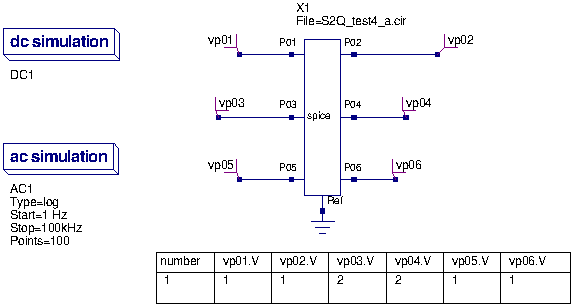
\includegraphics[width=0.8\linewidth]{S2Q_test4_a}
  \caption{March 22: SPICE to Qucs conversion: Test4 schematic plus dc output table for SPICE 2g6 and 3f5 linear capacitors test}
  \label{fig:S2Qtest4_1}
\end{figure} 

 \begin{flushleft} 

\tutsection{History of simulation results}
\tutsubsection{March 22 2007, Simulation tests by Mike Brinson}

A: SPICE 2g6 and 3f5 linear capacitor dc tests:

\begin{itemize}
 \item Vp01.V: \textbf{FAIL}; correct dc output = 0V.
 \item Vp02.V: \textbf{FAIL}; correct dc output = 0V.
 \item Vp03.V: \textbf{FAIL}; correct dc output = 1V.
 \item Vp04.V: \textbf{FAIL}; correct dc output = 1V.
 \item Vp05.V: \textbf{FAIL}; correct dc output = 1V.
 \item Vp06.V: \textbf{FAIL}; correct dc output = 1V.
 \end{itemize}


NOTE: It would appear that the value of a branch AC voltage source is being added to DC sources in the same branch during the DC simulation. This is incorrect. Qucs correctly computes the DC conditions from a schematic, see Fig.~\ref{fig:S2Qtest4_2}.   ERROR in SPICE to Qucs conversion process.
 
\end{flushleft} 

\begin{figure}
  \centering
  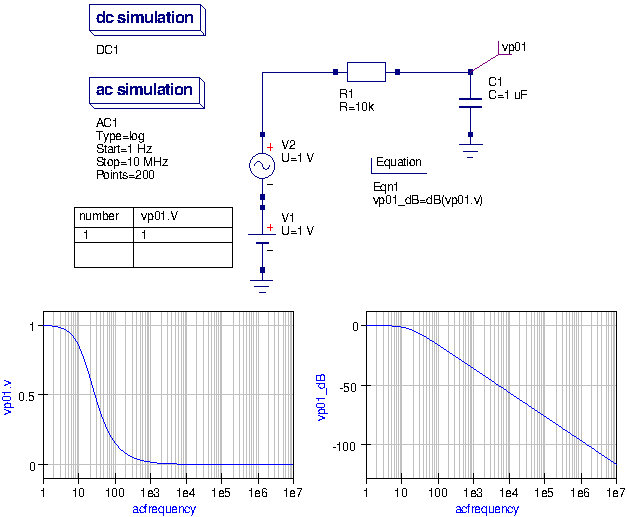
\includegraphics[width=0.8\linewidth]{S2Q_test4_a_1}
  \caption{March 22: Qucs RC simulation with series AC and DC sources}
  \label{fig:S2Qtest4_2}
\end{figure} 

\newpage 
Qucs netlist:
\begin{lstlisting}[
 language=Clean, 
 basicstyle=\small]
# Qucs 0.0.11  /media/hda2/S2Q_test4_prj/S2Q(test4_a).sch

.Def:S2Q_test4_a_cir _netP01 _netP02 _netP03 _netP04 _netP05
 _netP06 _ref
  .Def:S2Q_TEST4_A _ref _netP01 _netP02 _netP03 _netP04 
_netP05 _netP06
  Vac:V4 _net8 _cnet5 U="1V"
  Vac:V3 _net7 _cnet4 U="1V"
  Vac:V4AC _net6 _cnet3 U="1V"
  Vac:V3AC _net4 _cnet2 U="1V"
  Vac:V2 _net2 _cnet1 U="1V"
  Vac:V1 _net1 _cnet0 U="1V"
  Vdc:V1 _cnet0 _ref U="1"
  R:R1 _net1 _netP01 R="10k"
  C:C1 _netP01 _ref C="1u"
  Vdc:V2 _cnet1 _ref U="1"
  R:R3 _net2 _netP02 R="10k"
  C:C2 _netP02 _ref C="1u" V="10V"
  Vdc:V3DC _net3 _ref U="1V"
  Vdc:V3AC _cnet2 _net3 U="1"
  R:R4 _net4 _netP03 R="10k"
  C:C3 _netP03 _ref C="1u"
  Vdc:V4DC _net5 _ref U="1V"
  Vdc:V4AC _cnet3 _net5 U="1"
  R:R5 _net6 _netP04 R="10k"
  C:C4 _netP04 _ref C="1u" V="10V"
  Vdc:V3 _cnet4 _ref U="1V"
  R:R6 _net7 _netP05 R="10k"
  C:C5 _netP05 _ref C="1u"
  Vdc:V4 _cnet5 _ref U="1V"
  R:R7 _net8 _netP06 R="10k"
  C:C6 _netP06 _ref C="1u" V="10V"
  .Def:End
  Sub:X1 _ref _netP01 _netP02 _netP03 _netP04 _netP05 _netP06
 Type="S2Q_TEST4_A"
.Def:End


.DC:DC1 Temp="26.85" reltol="0.001" abstol="1 pA" vntol="1 uV" 
saveOPs="no" MaxIter="150" saveAll="no" convHelper="none" Solver="CroutLU"
Sub:X1 vp01 vp02 vp03 vp04 vp05 vp06 gnd Type="S2Q_test4_a_cir"

\end{lstlisting}



\begin{flushleft}
\newpage 
B: SPICE 2g6 and 3f5 linear capacitor ac tests:


Simulation waveforms appear to be correct, see Fig.~\ref{fig:S2Qtest4_3}.

\begin{figure}
  \centering
  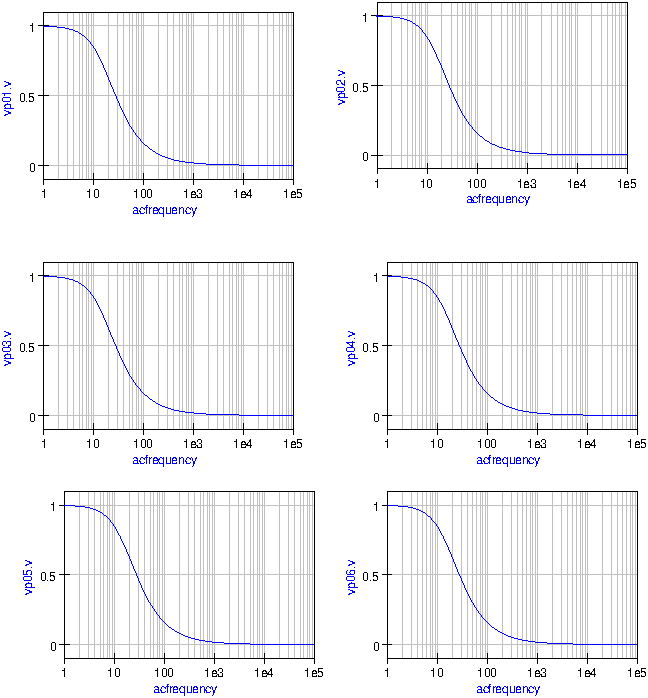
\includegraphics[width=0.8\linewidth]{S2Q_test4_a_2}
  \caption{March 22: Output waveforms for ac tests}
  \label{fig:S2Qtest4_3}
\end{figure} 

\end{flushleft}


\begin{flushleft}
C: SPICE 2g6 and 3f5 capacitor pulse tests.


SPICE code: File \verb|S2Q_test4_b.cir|

\begin{figure}
  \centering
  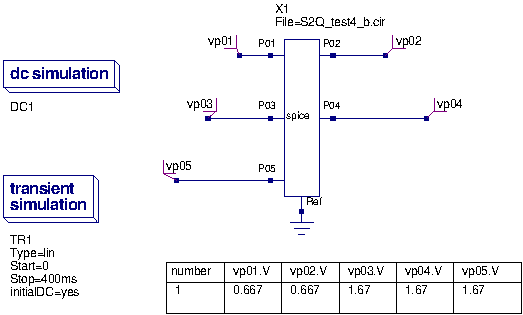
\includegraphics[width=0.8\linewidth]{S2Q_test4_b_1}
  \caption{March 22: SPICE to Qucs conversion: Test4 schematic plus dc output table for SPICE 2g6 and 3f5 linear capacitors pulse test}
  \label{fig:S2Qtest4_4}
\end{figure} 


\end{flushleft}

Qucs netlist:
\begin{lstlisting}[
 language=Clean, 
 basicstyle=\small]
# Qucs 0.0.11  /media/hda2/S2Q_test4_prj/S2Q(test4_b).sch

.Def:S2Q_test4_b_cir _netP01 _netP02 _netP03 _netP04 _netP05 _ref
  .Def:S2Q_TEST4_B _ref _netP01 _netP02 _netP03 _netP04 _netP05
  Vrect:V5 _net7 _cnet4 U="1" Td="50ms" Tr="1us" Tf="1us" 
  TH="0.100002" TL="0.049998"
  Vrect:V4AC _net6 _cnet3 U="1" Td="50ms" Tr="1us" Tf="1us" 
  TH="0.100002" TL="0.049998"
  Vrect:V3AC _net4 _cnet2 U="1" Td="50ms" Tr="1us" Tf="1us" 
  TH="0.100002" TL="0.049998"
  Vrect:V2 _net2 _cnet1 U="1" Td="50ms" Tr="1us" Tf="1us" 
  TH="0.100002" TL="0.049998"
  Vrect:V1 _net1 _cnet0 U="1" Td="50ms" Tr="1us" Tf="1us" 
  TH="0.100002" TL="0.049998"
  Vdc:V1 _cnet0 _ref U="0"
  R:R1 _net1 _netP01 R="10k"
  C:C1 _netP01 _ref C="1u" V="0V"
  Vdc:V2 _cnet1 _ref U="0"
  R:R3 _net2 _netP02 R="10k"
  C:C2 _netP02 _ref C="1u" V="-1V"
  Vdc:V3DC _net3 _ref U="1V"
  Vdc:V3AC _cnet2 _net3 U="0"
  R:R4 _net4 _netP03 R="10k"
  C:C4 _netP03 _ref C="1u" V="0V"
  Vdc:V4DC _net5 _ref U="1V"
  Vdc:V4AC _cnet3 _net5 U="0"
  R:R5 _net6 _netP04 R="10k"
  C:C5 _netP04 _ref C="1u" V="-1V"
  Vdc:V5 _cnet4 _ref U="1"
  R:R6 _net7 _netP05 R="10k"
  C:C6 _netP05 _ref C="1u" V="-1V"
  .Def:End
  Sub:X1 _ref _netP01 _netP02 _netP03 _netP04 _netP05 Type="S2Q_TEST4_B"
.Def:End


.DC:DC1 Temp="26.85" reltol="0.001" abstol="1 pA" vntol="1 uV" 
 saveOPs="no" MaxIter="150"
 saveAll="no" convHelper="none" Solver="CroutLU"
.TR:TR1 Type="lin" Start="0" Stop="400ms" Points="1000" 
 IntegrationMethod="Gear"Order="6" InitialStep="0.01 ns" 
 MinStep="1e-16" MaxIter="1500" reltol="0.001" abstol="100 pA" 
 vntol="100 uV" Temp="26.85" LTEreltol="1e-3" LTEabstol="1e-6" 
 LTEfactor="1" Solver="CroutLU" relaxTSR="no" initialDC="yes" 
 MaxStep="0"
Sub:X1 vp01 vp02 vp03 vp04 vp05 gnd Type="S2Q_test4_b_cir"

\end{lstlisting}
C 1: DC simulation.
\begin{itemize}
 \item Vp01.V: \textbf{FAIL}; correct dc output = 0V.
 \item Vp02.V: \textbf{FAIL}; correct dc output = 0V.
 \item Vp03.V: \textbf{FAIL}; correct dc output = 1V.
 \item Vp04.V: \textbf{FAIL}; correct dc output = 1V.
 \item Vp05.V: \textbf{FAIL}; correct dc output = 1V.
 \end{itemize}

NOTE: There appears to be an error in the dc simulation of the converted SPICE test netlist.  All dc output values have roughly 0.67 volts added to their correct value.  This could possibly be due to the way capacitor voltages are initialised. Qucs appears not to initialise capacitor voltages and they appear to be left floating after the SPICE to Qucs conversion process if they are not set by an IC=INCD statement?  Although SPICE allows capacitor voltages to be initialised via the optional parameter IC =INCOND this is only used at the start of transient analysis. The question is does it also get used in an .op dc analysis?  Here there is a problem for Qucs and possibly the best solution would be for Qucs to use the IC=INCOD value for the initial capacitor voltage, if given, otherwise set capacitor dc voltages to zero at the start of dc and transient analysis. Moreover, they must be initialised and NOT left floating at an indeterminate value.

\begin{flushleft}

C 2: Transient simulation:


Simulation waveforms appear to be correct, see Fig.~\ref{fig:S2Qtest4_5}.
NOTE: The transient analysis is set to use capacitor initilalisation voltages.


\begin{figure}
  \centering
  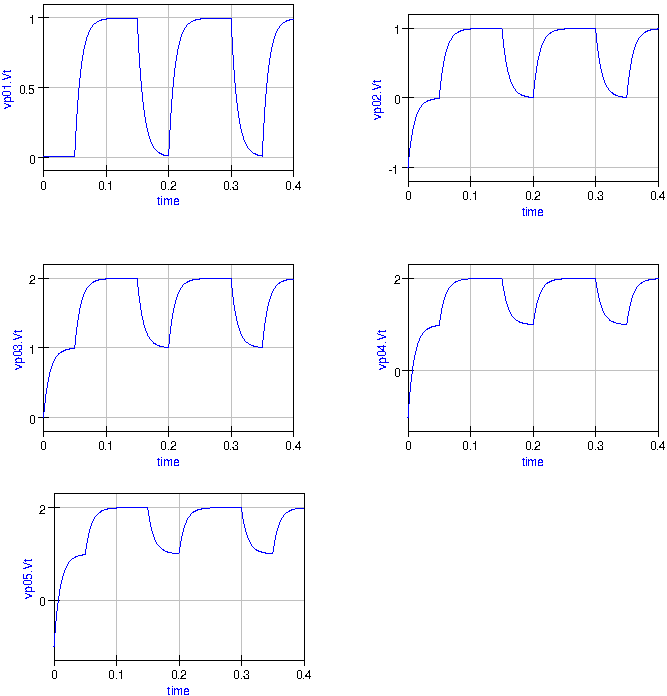
\includegraphics[width=0.8\linewidth]{S2Q_test4_b_2}
  \caption{March 22: Pulse test waveforms for SPICE 2g6 and 3f5 linear capacitors}
  \label{fig:S2Qtest4_5}
\end{figure} 
\end{flushleft}
\newpage 
\begin{flushleft}
 D: Combined DC, AC and transient source test.

SPICE code: File \verb|S2Q_test4_c.cir|

\begin{lstlisting}[
 language=Clean, 
 basicstyle=\footnotesize]
* SPICE to Qucs syntax test file 
* SPICE 2g6 and 3f5 capacitors.
* Pulse  test with dc and ac source
* in series with pulse voltage source.
*
.subckt S2Q_test4_c p06
*
v6 8 0 dc 1v ac 1v pulse(0 1 50ms 1us 1us 100ms 200ms)
r7 8 p06 10k
c7 p06 0 1u ic = -1v 
.ends
.end
\end{lstlisting} 

\end{flushleft}

\begin{flushleft}
 \begin{itemize}
 \item Vp06.V: \textbf{FAIL}; correct dc output = 1V.
 \item Vp06.v: \textbf{PASS}; correct ac waveform.
 \item Vp06.Vt: \textbf{FAIL}; Transient simulation will not run.
 
 \end{itemize}


\vspace{8mm}
NOTE: Vp06.Vt: If \textbf{ac 1v} is removed from voltage source statement, v6, the transient analysis gives correct result. Cause unknown.
\end{flushleft}


\begin{figure}
  \centering
  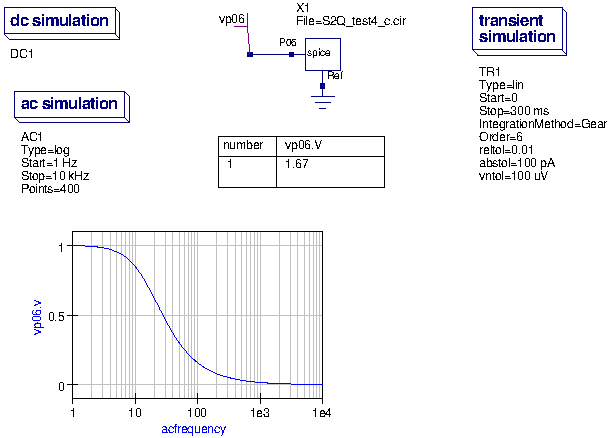
\includegraphics[width=0.8\linewidth]{S2Q_test4_b_3}
  \caption{March 22: Test circuit for combined dc, ac and pulse source test}
  \label{fig:S2Qtest4_6}
\end{figure} 

\newpage 
Qucs netlist:
\begin{lstlisting}[
 language=Clean, 
 basicstyle=\footnotesize]
# Qucs 0.0.11  /media/hda2/S2Q_test4_prj/S2Q(test4_c).sch

.Def:S2Q_test4_c_cir _netP06 _ref
  .Def:S2Q_TEST4_C _ref _netP06
  Vrect:V6 _net8 _cnet1 U="1" Td="50ms" Tr="1us" Tf="1us" TH="0.100002" 
  TL="0.049998"
  Vac:V6 _cnet1 _cnet0 U="1V"
  Vdc:V6 _cnet0 _ref U="1"
  R:R7 _net8 _netP06 R="10k"
  C:C7 _netP06 _ref C="1u" V="-1V"
  .Def:End
  Sub:X1 _ref _netP06 Type="S2Q_TEST4_C"
.Def:End


Sub:X1 vp06 gnd Type="S2Q_test4_c_cir"
.DC:DC1 Temp="26.85" reltol="0.001" abstol="1 pA" vntol="1 uV" saveOPs="no" 
MaxIter="150" saveAll="no" convHelper="none" Solver="CroutLU"
.AC:AC1 Type="log" Start="1 Hz" Stop="10 kHz" Points="400" Noise="no"
.TR:TR1 Type="lin" Start="0" Stop="300 ms" Points="300" IntegrationMethod="Gear"
 Order="6" InitialStep="0.001 ns" MinStep="1e-16" MaxIter="150" reltol="0.01" 
abstol="100 pA" vntol="100 uV" Temp="26.85" LTEreltol="1e-3" LTEabstol="1e-6" 
LTEfactor="1" Solver="CroutLU" relaxTSR="no" initialDC="yes" MaxStep="0"

\end{lstlisting} 






\begin{flushleft}
E: SPICE 2g6 non-linear capacitor tests.
\linebreak 
NO results - Qucs 0.0.11 does  not allow non-linear capacitors of the SPICE 2g6 form.  Nonlinear capacitors will be added to both Qucs and QUCSCONV sometime in the future when the nonlinear independent voltage and current sources are implemented, see the todo list..
\vspace*{5mm}
\linebreak
F: SPICE 3f5 tests
SPICE code: File \verb|S2Q_test4_e.cir|

\begin{lstlisting}[
 language=Clean, 
 basicstyle=\footnotesize]
* SPICE to Qucs syntax test file 
* SPICE 3f5 semiconductor capacitors.
* DC and AC tests.
*
.subckt S2Q_test4_e p01 p02 p03 p04 p05 p06
v1 1 0 DC 1v AC 1v
r1 1 p01 10k
c1 p01 0 1u
*

v2 2 0 dc 1v ac 1v
r3 2 p02  10k
c2 p02 0 1u ic = 10v
*
v3dc 3 0 dc 1v
v3ac 4 3 ac 1v
r4 4 p03  10k
c3 p03 0 1u ic = -10v
*
v4dc 5 0 dc 1v
v4ac 6 5 ac 1v
r5 6 p04  10k
c4 p04 0  cmod1 L=10u W=1u 
.model cmod1 C(CJ=50u CJSW=20p NARROW=0.1u)
*
v3 7 0 dc 1v ac 1v
r6 7 p05  10k
c5 p05 0 cmod1 L=10u W=1u
*
v4 8 0 dc 1v ac 1v
r7 8 p06  10k
c6 p06 0 cmod2 L=10u
.model cmod2 C(DEFW=1u CJ=50u CJSW=20p NARROW=0.1u)
.ends
.end
\end{lstlisting} 
\end{flushleft}

\begin{flushleft}
 


Qucs netlist (DC simulation)
\begin{lstlisting}[
 language=Clean, 
 basicstyle=\footnotesize]
# Qucs 0.0.11  /media/hda2/S2Q_test4_prj/S2Q(test4_e).sch

.Def:S2Q_test4_e_cir _netP01 _netP02 _netP03 _netP04 _netP05 _netP06 _ref
  .Def:S2Q_TEST4_E _ref _netP01 _netP02 _netP03 _netP04 _netP05 _netP06
  Vac:V4 _net8 _cnet5 U="1V"
  Vac:V3 _net7 _cnet4 U="1V"
  Vac:V4AC _net6 _cnet3 U="1V"
  Vac:V3AC _net4 _cnet2 U="1V"
  Vac:V2 _net2 _cnet1 U="1V"
  Vac:V1 _net1 _cnet0 U="1V"
  Vdc:V1 _cnet0 _ref U="1V"
  R:R1 _net1 _netP01 R="10k"
  C:C1 _netP01 _ref C="1u"
  Vdc:V2 _cnet1 _ref U="1V"
  R:R3 _net2 _netP02 R="10k"
  C:C2 _netP02 _ref C="1u" V="10V"
  Vdc:V3DC _net3 _ref U="1V"
  Vdc:V3AC _cnet2 _net3 U="1"
  R:R4 _net4 _netP03 R="10k"
  C:C3 _netP03 _ref C="1u" V="-10V"
  Vdc:V4DC _net5 _ref U="1V"
  Vdc:V4AC _cnet3 _net5 U="1"
  R:R5 _net6 _netP04 R="10k"
  C:C4 _netP04 _ref L="10u" W="1u" C="1e-12"
  Vdc:V3 _cnet4 _ref U="1V"
  R:R6 _net7 _netP05 R="10k"
  C:C5 _netP05 _ref L="10u" W="1u" C="1e-12"
  Vdc:V4 _cnet5 _ref U="1V"
  R:R7 _net8 _netP06 R="10k"
  C:C6 _netP06 _ref L="10u" C="1e-12"
  .Def:End
  Sub:X1 _ref _netP01 _netP02 _netP03 _netP04 _netP05 _netP06 Type="S2Q_TEST4_E"
.Def:End

Sub:X1 vp01 vp02 vp03 vp04 vp06 vp07 gnd Type="S2Q_test4_e_cir"
.DC:DC1 Temp="26.85" reltol="0.001" abstol="1 pA" vntol="1 uV"  
 saveOPs="no" MaxIter="150" saveAll="no" convHelper="none" Solver="CroutLU"

\end{lstlisting} 
\begin{verbatim}

RESULTS:
line 25: checker error, extraneous property `L' is invalid in `C:C4' 
line 25: checker error, extraneous property `W' is invalid in `C:C4' 
line 28: checker error, extraneous property `L' is invalid in `C:C5' 
line 28: checker error, extraneous property `W' is invalid in `C:C5' 
line 31: checker error, extraneous property `L' is invalid in `C:C6' 
\end{verbatim}  
Errors in SPICE semiconductor capacitor to Qucs netlist format conversion.
\end{flushleft}


\tutsubsection{March 25 2007, Simulation tests by Mike Brinson}


\begin{flushleft}
 Code modifications:
\begin{itemize}
 \item *\verb| check_spice.cpp|: Handling capacitor models correctly.
        Also fixed wrong DC value of sources when neither the DC
        directive nor an immediate value was given. Stefan Jahn.
\end{itemize}

A: SPICE 2g6 and 3f5 linear capacitor dc tests:

\begin{itemize}
 \item Vp01.V: \textbf{PASS}; dc output = 0V.
 \item Vp02.V: \textbf{PASS}; dc output = 0V.
 \item Vp03.V: \textbf{PASS}; dc output = 1V.
 \item Vp04.V: \textbf{PASS}; dc output = 1V.
 \item Vp05.V: \textbf{PASS}; dc output = 1V.
 \item Vp06.V: \textbf{PASS}; dc output = 1V.
 \end{itemize}

\end{flushleft}



\begin{flushleft}
 C: SPICE code: \verb|File S2Q_test4_b.cir|

Further notes on test results:
\begin{itemize}
 \item SPICE independent voltage sources with DC, AC and transient elements appear to be handled differently by SPICE and Qucs. In a SPICE DC operating point simulation, time domain sources have their DC values set to their value at simulation time equal to zero seconds. However, for time domain  pulse source Qucs finds the DC level by integrating it's waveform over one signal cycle. This results in a DC value of 0.6667V, yielding the DC offset recorded in the original test. In Qucs a generator is added to the Qucs netlist for each of the elements specified in the original SPICE voltage source entry.  Hence, it is possible to have upto three voltage sources in series. Figure~\ref{fig:S2Qtest4_7} illustrates that the DC offset occurs from a pulse generator placed in series with a DC source on a schematic.
 \item The same comment concerning SPICE and Qucs differences introduced above applies to the AC component of a SPICE independent voltage source component.  In this case there is not a DC offset but because the frequency of the source is NOT included in the SPICE code, Qucs assumes it's default value to be 1GHz.  Hence, in the time domain an AC generator is included in the independent voltage source  branch with a frequency of 1GHz.  This in turn causes the transient analysis routines to require a very small time step for satisfactory accuracy and hence the simulation takes a long time and appears to hang. SPICE on the other hand considers the AC source to be only applicable to small signal AC analysis and does NOT include it in time domain simulation. Yet another example of the difference between SPICE and Qucs. 
 \item RECOMMENDATIONS:
\begin{enumerate}
 \item Mix DC, AC and time domain source elements in SPICE independent voltage sources with care when converting code to be simulated with Qucs.
 \item When simulating SPICE netlists in the time domain ensure capacitors have their initial condition voltages set to known values. This ensures that the correct DC conditions form the starting point for a transient circuit simulation.
\end{enumerate}

\end{itemize}

\end{flushleft}



\begin{figure}
  \centering
  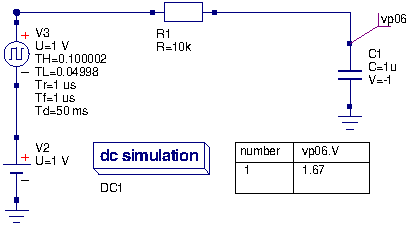
\includegraphics[width=0.8\linewidth]{test_dc_pulse}
  \caption{March 25: DC simulation showing 0.6667V offset}
  \label{fig:S2Qtest4_7}
\end{figure} 

\begin{flushleft}
F: SPICE 3f5 tests
SPICE code: File \verb|S2Q_test4_e.cir|
\linebreak 
DC simulation test: All outputs \textbf{PASS }with a DC value of 1V.
\end{flushleft}

\tutsection{References}
\begin{enumerate}
 \item A. Vladimirescu, Kaihe Zhang, A.R. Newton, D.O Pederson A. Sangiovanni-Vincentelli, SPICE 2G User's Guide (10 Aug 1981), Department of Electrical Engineering and Computer Sciences, University of California, Berkeley, Ca., 94720.
\item B. Johnson, T. Quarles, A.R. Newton, P.O. Pederson, A.Sangiovanni-Vincentelli, SPICE3 Version 3f User's Manual (October 1972),  Department of Electrical Engineering and Computer Sciences, University of California, Berkeley, Ca., 94720.
\item Andrei Vladimirescu, THE SPICE book,1994, John Wiley and Sons. Inc., ISBN 0-471-609-26-9.
\end{enumerate}


